\documentclass{article}
\usepackage[english,russian]{babel}
\usepackage{textcomp}
\usepackage{geometry}
  \geometry{left=2cm}
  \geometry{right=1.5cm}
  \geometry{top=1.5cm}
  \geometry{bottom=2cm}
\usepackage{tikz}
\usepackage{multicol}
\usepackage{hyperref}
\usepackage{listings}
\pagenumbering{gobble}

\lstdefinestyle{csMiptCppStyle}{
  language=C++,
  basicstyle=\linespread{1.1}\ttfamily,
  columns=fixed,
  fontadjust=true,
  basewidth=0.5em,
  keywordstyle=\color{blue}\bfseries,
  commentstyle=\color{gray},
  texcl=true,
  stringstyle=\ttfamily\color{orange!50!black},
  showstringspaces=false,
  numbersep=5pt,
  numberstyle=\tiny\color{black},
  numberfirstline=true,
  stepnumber=1,      
  numbersep=10pt,
  backgroundcolor=\color{white},
  showstringspaces=false,
  captionpos=b,
  breaklines=true
  breakatwhitespace=true,
  xleftmargin=.2in,
  extendedchars=\true,
  keepspaces = true,
  tabsize=4,
  upquote=true,
  frame=none,
  emph={if, else, elif, endif, include, define, defined},
  emphstyle={\color{blue}},
  literate=*{\#}{{\textcolor{blue}{\#}}}{1},
}


\lstdefinestyle{csMiptCppLinesStyle}{
  style=csMiptCppStyle,
  frame=lines,
}

\lstdefinestyle{csMiptCppBorderStyle}{
  style=csMiptCppStyle,
  framexleftmargin=5mm, 
  frame=shadowbox, 
  rulesepcolor=\color{gray}
}


\lstdefinestyle{csMiptBash}{
breaklines=true,
frame=tb,
language=bash,
breakatwhitespace=true,
alsoletter={*()"'0123456789.},
alsoother={\{\=\}},
basicstyle={\ttfamily},
keywordstyle={\bfseries},
literate={{=}{{{=}}}1},
prebreak={\textbackslash},
sensitive=true,
stepnumber=1,
tabsize=4,
morekeywords={echo, function},
otherkeywords={-, \{, \}},
literate={\$\{}{{{{\bfseries{}\$\{}}}}2,
upquote=true,
frame=none
}




\lstset{style=csMiptCppLinesStyle}
\lstset{literate={~}{{\raisebox{0.5ex}{\texttildelow}}}{1}}


\renewcommand{\thesection}{\arabic{section}}
\makeatletter
\def\@seccntformat#1{\@ifundefined{#1@cntformat}%
   {\csname the#1\endcsname\quad}%    default
   {\csname #1@cntformat\endcsname}}% enable individual control
\newcommand\section@cntformat{Часть \thesection:\space}
\makeatother




\begin{document}
\title{Семинар \#1: Компиляция и линковка \vspace{-5ex}}\date{}\maketitle

В данном семинаре рассматриваются процессы компиляции и линковки, а также создание и использование статических и динамических библиотек. Процессы компиляции и линковки могут существенно различаться в зависимости от операционной системы. Кроме того, компиляция и линковка на языке C++ имеют свои особенности по сравнению с языком C.
Поэтому в этом семинаре сначала будут рассмотрены основные этапы компиляции и линковки в операционной системе Linux на языке C. Затем будут подробно разобраны особенности этих процессов в языке C++. В завершение будут освещены ключевые отличия и специфика компиляции и линковки в операционной системе Windows.

\section{Этапы компиляции}
\begin{description}
\item[Компиляция] -- то процесс преобразования исходного кода, в машинный код, который может быть выполнен компьютером. Компилятор -- это программа, которая осуществляет компиляцию. \\
В этом курсе мы использовали компилятор \texttt{gcc} для кода на языке C и компилятор \texttt{g++} для кода на C++.
\end{description}


\noindent Компиляция состоит из четырех основных этапов: препроцессинг, компиляция, ассемблирование и линковка. Если использовать компилятор \texttt{gcc}, просто передав ему имя файла командой:
\begin{lstlisting}[style=csMiptBash]
$ gcc main.c
\end{lstlisting}
то все этапы будут выполнены автоматически, и на выходе получится готовый исполняемый файл. Однако при необходимости можно выполнить только отдельные этапы компиляции, чтобы более детально контролировать процесс. Например, можно остановиться после препроцессинга или после генерации объектного файла.

\begin{enumerate}
\item \textbf{Препроцессинг}
\begin{list}{$\circ$}{}  
\item На этом этапе выполняется обработка директив препроцессора (\texttt{\#include}, \texttt{\#define}, \texttt{\#ifdef} и т.д.)
\item Происходит включение заголовочных файлов, раскрытие макросов и удаление комментариев.
\item Выполнить только этот этап компиляции с помощью \texttt{gcc} можно следующим образом:
\begin{lstlisting}[style=csMiptBash]
$ gcc -E main.c -o main.i
\end{lstlisting}
\end{list}

\item \textbf{Компиляция} (не путать с компиляцией, состоящей из четырёх этапов)
\begin{list}{$\circ$}{}  
\item Преобразованный на этапе препроцессинга код компилируется в ассемблерный код.
\item Результатом этого этапа является является файл с расширением \texttt{.s}.
\item Выполнить процесс компиляции до этого этапа включительно можно следующей командой:
\begin{lstlisting}[style=csMiptBash]
$ gcc -S -masm=intel main.c
\end{lstlisting}
\end{list}

\item \textbf{Ассемблирования}
\begin{list}{$\circ$}{}  
\item Ассемблерный код преобразуется в объектный код (машинный код), который представляет собой набор инструкций для процессора.
\item Результатом этого этапа является объектный файл с расширением \texttt{.o}.
\item Выполнить процесс компиляции до этого этапа включительно можно следующей командой:
\begin{lstlisting}[style=csMiptBash]
$ gcc -c main.c
\end{lstlisting}
\end{list}

\item \textbf{Линковка}
\begin{list}{$\circ$}{}  
\item На этом этапе все объектные файлы и библиотеки связываются вместе. 
\item Результатом этого этапа является исполняемый файл (на Linux исполняемые файлы обычно не имеют расширения, на Windows исполняемые файлы имеют расширение \texttt{.exe}) или библиотека.
\end{list}
\end{enumerate}


Предположим, что наш проект состоит из одного файла \texttt{main.c} и из библиотек использует только стандартную библиотеку C и только функции из \texttt{stdio.h} (например,  \texttt{printf}). Тогда процесс компиляции такого проекта можно показать на следующей схеме:\\

\begin{center}
\includegraphics[scale=0.8]{../images/01stages.png}
\end{center}

\begin{itemize}
\item На этапе препроцессинга компилятор видит директиву \texttt{\#include <stdio.h>}. Поэтому он приступает к поиску заголовочного файла \texttt{stdio.h} в стандартных путях. Стандартные пути, в которых нужно искать заголовочные файлы хранятся внутри компилятора, их можно увидеть с помощью команды:
\begin{lstlisting}[style=csMiptBash]
$ echo | gcc -E -v -
\end{lstlisting}
\item После того как он найдёт файл, он за место строки \texttt{\#include <stdio.h>} вставит содержимое этого файла. 

\item Файл \texttt{stdio.h} содержит код на языке C и внутри этого файла также могут быть директивы \texttt{\#include}, \texttt{\#define} и другие. Компилятор будет выполнять все директивы пока их не останется.

\item Внутри файла \texttt{stdio.h} НЕ содержатся коды стандартных функций. Там содержатся объявления (прототипы) функций. Это нужно, чтобы наша программа знала, что существуют те или иные функции.

\item Код стандартных функций в уже скомпилированном виде (так называемый машинный код) содержится в библиотеке \texttt{libc.so.6} и подключается на этапе линковки.

\item Различают статическую и динамическую линковку. При статической линковке машинный код всех используемых функций вставляется в окончательный исполняемый файл. При динамической линковке необходимые функции находятся в библиотеках во время выполнения.

\end{itemize}


\newpage
\section{Разделение кода программы на части с помощью \texttt{\#include}}
Простейшей способ разделение кода программы на несколько файлов -- это использование директивы \texttt{\#include}.

\begin{center}
\includegraphics[scale=0.85]{../images/02main_cube_include.png}
\end{center}
Файл \texttt{cube.h} просто вставится в файл \texttt{main.c} за место строки \texttt{\#include "cube.h"} на этапе препроцессинга. При использовании угловых \texttt{<>} скобок в \texttt{\#include} компилятор будет искать файл в стандартных путях, а при использовании кавычек \texttt{"{}"} сначала поищет в текущей директории. 
Скомпилировать эту программу можно так:
\begin{lstlisting}[style=csMiptBash]
$ gcc main.c
\end{lstlisting}
Передавать название файла \texttt{cube.h} компилятору не нужно, так как он найдёт этот файл через \texttt{\#include}. Процесс компиляции этой программы почти не будет отличатся от предыдущей, что можно увидеть на схеме:\\

\begin{center}
\includegraphics[scale=0.7]{../images/03stages_cube_include.png}
\end{center}

\section{Раздельная компиляция}
\begin{description}
\item[Раздельная компиляция] -- это подход, при котором программа разбивается на несколько отдельных файлов исходного кода (\texttt{.c}), которые компилируются независимо друг от друга. В отличии от использования \texttt{\#include} при раздельной компиляции части программы будут компилироваться отдельно и объединяться вместе только на этапе линковки. 
\end{description}

\subsection*{Ошибочный подход}
Попробуем произвести раздельную компиляцию нашей программы, просто разделив один файл исходного кода на два: \texttt{main.c} и \texttt{cube.c} и передав на вход компилятору эти два файла.
\begin{center}
\includegraphics[scale=0.85]{../images/04main_cube_separate1.png}
\end{center}
Попробуем скомпилировать программу следующей командой:
\begin{lstlisting}[style=csMiptBash]
$ gcc main.c cube.c
\end{lstlisting}
Произойдёт следующая ошибка:
\begin{verbatim}
main.c:5:20: error: implicit declaration of function 'cube'
\end{verbatim}
Ошибка происходит из-за того, что компилятор пытается скомпилировать файлы \texttt{main.c} и \texttt{cube.c} раздельно, но не может скомпилировать файл \texttt{main.c} из-за того, что встечает неизвестную ему функцию \texttt{cube}. Компилятор не знает, что такая функция существует в другом файле, так как он должен скомпилировать два файла независимо друг от друга. Узнать, что в другом файле есть функция \texttt{cube} компилятор сможет только на этапе линковки.
\subsection*{Более правильный подход}
Мы можем сказать компилятору, что функция \texttt{cube} существует в другом файле программы, просто объявив (написав прототип) эту функцию в файле \texttt{main.c}.
\begin{center}
\includegraphics[scale=0.85]{../images/05main_cube_separate2.png}
\end{center}
В этом случае, при компилировании файла \texttt{main.c} компилятор будет знать, что функция \texttt{cube} существует и компиляция пройдёт успешно.

\subsection*{Использование заголовочных файлов}
Обычно, код делится на части таким образом, что в каждом файле исходного кода содержится множество функций, а не одна, как в нашем примере. Представьте, что за место файла \texttt{cube.c} с одной функцией, у нас был бы файл \texttt{mathfuncs.c}, который бы содержал 100 разных математических функций. Чтобы подключить такой файл к файлу \texttt{main.c} нам нужно было бы написать 100 прототипов функций в файле \texttt{main.c}. Если бы нам потребовалось подключить файл \texttt{mathfuncs.c} к ещё одному файлу, то нам бы потребовалось написать все 100 прототипов ещё раз. Чтобы решить эту проблему используются заголовочные файлы.

\begin{description}
\item[Заголовочный файл] (англ. \textit{header file}) -- это текстовый файл с расширением \texttt{.h}, который содержит объявления функций, глобальных переменных, макросы, объявления структур и других типов данных, предназначенных для использования в нескольких файлах исходного кода (\texttt{.c}). Такие файлы вставляются в файлы исходного кода с помощью \texttt{\#include}.
\end{description}

\begin{center}
\includegraphics[scale=0.85]{../images/06main_cube_separate3.png}
\end{center}
Теперь, если даже у нас будет файл, содержащий не одну функцию, а 100 функций, то мы просто напишем соответствующий заголовочный файл, содержащий 100 прототипов функций, и будем использовать его для подключения к другим файлам.

\noindent Скомпилировать данную программу можно командой:
\begin{lstlisting}[style=csMiptBash]
$ gcc main.c cube.c
\end{lstlisting}
Указывать файл \texttt{cube.h} не нужно, так как компилятор найдёт его и вставит, используя директиву \texttt{\#include}.
При использовании этой команды компилятор выполнит все этапы компилирования и получит окончательный исполняемый файл. При этом компилятор будет компилировать файлы \texttt{main.c} и \texttt{cube.c} раздельно и объединять их только на этапе линковки.

Но можно произвести компиляцию поэтапно, воспользовавшись соответствующими опциями компилятора. Например, мы можем сами скомпилировать отдельно файл \texttt{main.c} в объектный файл \texttt{main.o}, а файл \texttt{cube.c} в объектный файл \texttt{cube.o}, а после этого слинковать их вместе в итоговый исполняемый файл.
\begin{lstlisting}[style=csMiptBash]
$ gcc -c main.c      # компилируем файл main.c отдельно и получаем файл main.o
$ gcc -c cube.c      # компилируем файл cube.c отдельно и получаем файл cube.o
$ gcc main.o cube.o  # линкуем файлы main.o и cube.o и получаем исполняемый файл
\end{lstlisting}

\subsubsection*{Замечание об использовании заголовочных файлов}
Как правило, файлы с расширением \texttt{.h} предназначения для того, чтобы содержать в себе только объявления (функций, структур, глобальных переменных) и макросы. Но несмотря на это, иногда в таких файлах содержится сам код функций (как мы это делали в Части 2). Это допустимо, но нужно понимать, что храня код функций в заголовочных файлах, мы лишаемся преимуществ, которые даёт раздельная компиляция.

\subsubsection*{Замечание о подключении заголовочного файла в соответствующий исходный файл}
Заголовочный файл следует подключать во все файлы, в которых используются его объявления. Более того, важно подключать заголовочный файл его в соответствующий \texttt{.c}-файл. Например, \texttt{cube.h} должен быть включён в \texttt{cube.c}. Хотя компиляция может пройти и без этого, такое подключение обеспечивает контроль соответствия объявлений и определений. Если изменить объявление в \texttt{cube.h}, но забыть обновить \texttt{cube.c}, компилятор сразу обнаружит ошибку. Правильное разделение кода в нашем примере выглядит так:
\begin{center}
\includegraphics[scale=0.85]{../images/06main_cube_separate3b.png}
\end{center}



\subsubsection*{Схема процесса раздельной компиляции нашей программы:}
\begin{center}
\includegraphics[scale=0.7]{../images/07stages_cube_separate.png}
\end{center}





\newpage
\subsection*{Преимущества раздельной компиляции}
Само по себе разбиение программы на несколько файлов умеет преемущества, такие как:
\begin{itemize}
\item \textbf{Лучшая структура программы}\\
Программу, разделённую на несколько файлов, можно сделать более структурированной. Код разбивается на части, каждая из которых отвечает за определённую функциональность.
\item \textbf{Повторное использование кода}\\
Код из одного проекта легче использовать в других проектах.
\end{itemize}
Однако, разбить код на части можно, используя только директиву \texttt{\#include}, не прибегая к раздельной компиляции. Использование раздельной компиляции по сравнению с \texttt{\#include} имеет следующие преимущества:

\begin{itemize}
\item \textbf{Ускорение перекомпиляции после изменений}\\
Это самое главное преимущество раздельной компиляции. Чтобы его понять, представьте, что у вас есть большая программа, состоящая из сотен файлов. Предположим, что
мы сделали маленькое изменение в одном из файлов и хотим заново скомпилировать программу. Если бы мы не использовали раздельную компиляцию (а просто бы подключали через \texttt{\#include}), то нам бы пришлось перекомпилировать всю программу. Но, если мы используем раздельную компиляцию и сохранили объектные файлы со времени предыдущей компиляции, то нам будет достаточно перекомпилировать только файл, в котором были сделаны изменения. Этап линковки, всё же, придётся повторить для всей программы. Тем не менее, это всё равно будет намного быстрее компиляции всей программы.

\item \textbf{Более точная настройка компиляции}\\
Дальше в этом семинаре мы разберём, что компилировать программу можно разными способами, передавая компилятору разные опции. Использование раздельной компиляции позволяет использовать разные опции для разных файлов программы. Иногда это бывает полезно.
\end{itemize}


\subsection*{Ещё один пример программы, использующей раздельную компиляцию}
Рассмотрим немного более сложную программу:

\begin{center}
\includegraphics[scale=0.8]{../images/08another_separate.png}
\end{center}

\noindent
Разбить такую программу на несколько файлов, для последующего применения раздельной компиляции, можно следующим образом. Обратите внимание, что объявление структуры \texttt{Point} тоже помещается в заголовочный файл. Далее, мы включаем файл \texttt{point.h} во все файлы, где используется структура \texttt{Point}.
\begin{center}
\includegraphics[scale=0.8]{../images/09another_separate2.png}
\end{center}

\newpage
\section{Опции компиляции}
\begin{description}
\item[Опции компиляции] -- это параметры, которые передаются компилятору через командную строку для управления процессом компиляции. Они позволяют настраивать поведение компилятора, указывать пути к файлам, задавать уровни оптимизации, стандарты языка и многое другое.
\item[Флаги компиляции] -- формально это булевые опции компиляции. Но часто понятия флаги компиляции и опции компиляции используются как синонимы.
\end{description}

\subsection*{Опция \texttt{-o}, задающая название выходного файла}
Если скомпилировать программу, следующим образом:
\begin{lstlisting}[style=csMiptBash]
$ gcc main.c
\end{lstlisting}
то навыходе получится исполняемый файл под названием \texttt{a.out}. Запустить этот файл можно будет с помощью:
\begin{lstlisting}[style=csMiptBash]
$ ./a.out
\end{lstlisting}
Название итогового файла можно задать с помощью опции \texttt{-o}:
\begin{lstlisting}[style=csMiptBash]
$ gcc main.c -o dog
\end{lstlisting}
В этом случае создастся файл с именем \texttt{dog}. Запустить этот файл можно будет с помощью: 
\begin{lstlisting}[style=csMiptBash]
$ ./dog
\end{lstlisting}

\subsection*{Опции для выполнения только первых шагов компиляции}
\begin{itemize}
\item Опция \texttt{-E} -- компилятор исполнит только этап препроцессинга.
\item Опция \texttt{-S} -- компилятор исполнит этапы препроцессинга и компиляции.
\item Опция \texttt{-c} -- компилятор исполнит этапы препроцессинга, компиляции и ассемблирования.
\end{itemize}


\subsection*{Опции для выбора стандарта языка}
Язык C появился на свет в 1972 году и быстро стал популярным. В те времена было написано несколько компиляторов языка различными компаниями. Однако ранние компиляторы могли сильно различаться между собой. Можно сказать, что каждый компилятор воспринимал только свою версию языка, отличающуюся от тех с какими работали другие компиляторы. Это являлось большой проблемой, так как код, написанный для одного компилятора, мог не работать на другом. Для решения этой проблемы, в 1989 был представлен стандарт языка. Стандарт языка -- это документ, который полностью описывает язык и его стандартную библиотеку. После этого разработчики компиляторов стали ориентироваться на стандарт и различий между разными версиями языка для различных компиляторов стало меньше.

Первая версия языка C (вышедшая в 1972) и даже первая стандартизированная версия языка (вышедшая в 1989) сильно отличались от современного языка C. Со временем в язык добавлялись новые возможности. Таким образом, язык С (как и большинство других языков программирования) не является постоянным, а меняется во времени. Поэтому переодически выходят новые стандарты языка. Так, новые стандарты вышли в 1999-м, 2011-м и 2023-м годах. Грубо говоря, стандарты являются версиями языка программирования. Код, написанный в соответствии с одним стандартом, может не компилироваться под другой версией стандарта.

Выбор стандарта языка C в компиляторе \texttt{gcc} осуществляется с помощью опции \texttt{-std=версия\_стандарта}. Например, \texttt{-std=c89} означает, что нужно использовать стандарт 1989 года. Есть аналогичные опции \texttt{-std=c99}, \texttt{-std=c11} и \texttt{-std=c23} для стандартов 1999-го, 2011-го и 2023-го годов соответственно.

Аналогично, есть стандарты языка C++. Стандарты языка C++ выходили в 1998-м, 2003-м, 2011-м, 2014-м, 2017-и, 2020-м, 2023-м и 2026-м годах. Для языка C++ планируется выход нового стандарта каждые 3 года. Выбор стандарта языка C++ в компиляторе \texttt{g++} осуществляется с помощью следующих опций: \texttt{-std=c++98}, \texttt{-std=c++03}, \texttt{-std=c++11}, \texttt{-std=c++14}, \texttt{-std=c++17}, \texttt{-std=c++20}, \texttt{-std=c++23}, \texttt{-std=c++26}, ...

\subsection*{Опции для работы с предупреждениями (warnings)}
\begin{description}
\item[Предупреждение] (англ. \textit{warning}) -- это сообщение компилятора, которое указывает на потенциально проблемный код, который не нарушает синтаксических правил языка, но может привести к различным ошибкам во времени выполнения.
\end{description}
Формально, предупреждения не являются ошибками, поэтому программу, содержащую предупреждения, можно скомпилировать. Но к предупреждениям следует относится серьёзно, так как они могут указывать на ошибки в программе. Рассмотрим следующую программу, содержащую ошибку:
\begin{lstlisting}[style=csMiptCppStyle]
#include <stdio.h>
int main()
{
    for (int i = 0; i < 10; ++i);
        printf("Hello\n");
}
\end{lstlisting}
По умолчанию, данная программа скомпилируется без ошибок. Если её запустить, то на экране напечатается слово \texttt{Hello} один раз, что, скорей всего, не то, что мы хотели. Если же данную программу скомпилировать с опцией \texttt{-Wall}, то компилятор выдаст предупреждение -- лишняя точка с запятой после цикла \texttt{for}. Проверки на большинство предупреждений не включены по умолчанию. Чтобы их включить используются опции:

\begin{itemize}
\item \texttt{-Wall} -- включает некоторые предупреждения.
\item \texttt{-Wextra} -- включает дополнительные предупреждения.
\item \texttt{-Wconversion} -- предупреждает о неявных преобразованиях, которые могут привести к потере данных.
\item \texttt{-Werror} -- превращает все найденные предупреждения в ошибки.
\end{itemize}





\subsection*{Опции для оптимизации кода}
Оптимизация кода - это изменение программы для увеличения её производительности без изменения её наблюдаемого поведения. Компилятор может оптимизировать ваш код, если ему передать необходимые опции. Рассмотрим, например, следующую программу:
\begin{lstlisting}[style=csMiptCppStyle]
#include <stdio.h>
int main()
{
    int a = 0;
    for (int i = 0; i < 2000000000; ++i)
        a += 1;
    printf("%i\n", a);
}
\end{lstlisting}
Эта программа прибавляет к числу, изначально равному нулу, единицу 2 миллиарда раз, а затем печатает это число. Очевидно, что эту программу можно очень сильно оптимизировать, если просто убрать цикл из программы и просто напечатать на экран число \texttt{2000000000}.\\
Если скомпилировать эту программу без опций для оптимизации, то получится программа, которая будет честно выполнять весь цикл и, соответственно, очень долго работать. Если же использовать опцию оптимизации:
\begin{lstlisting}[style=csMiptBash]
$ gcc -O2 main.c
\end{lstlisting}
То комплятор оптимизирует программу. В результате программа не будет выполнять цикл, а просто напечатает на экран число \texttt{2000000000}. Такая программа будет работать очень быстро. 

Компилятор может производить множество оптимизаций, например, вычисление констант на этапе компиляции, разворачивание циклов, для уменьшения накладных расходов на проверку условия, замена вызова функции на её тело (инлайнинг) и многие другие. Для включения оптимизаций используются следующие опции:
\begin{itemize}
\item \texttt{-O0} -- отключает почти все оптимизации, используется по умолчанию.
\item \texttt{-O1} -- включает базовые оптимизации.
\item \texttt{-O2} -- включает большинство оптимизаций.
\item \texttt{-O3} -- включает все оптимизации, иногда может сильно увеличить размер исполняемого файла.
\item \texttt{-Os} -- пытается минимизировать размер исполняемого файла.
\end{itemize}


\subsection*{Опция \texttt{-g} для включения информации для дебаггера}



\subsection*{Опции, для определения макросов (определений компиляции)}
Рассмотрим следующую программу:
\begin{lstlisting}[style=csMiptCppStyle]
#include <stdio.h>

int main()
{
    #if defined(CAT)
        printf("Yes\n");
    #else
        printf("No\n");
    #endif
}
\end{lstlisting}
В данной программе директивы \texttt{\#if}, \texttt{\#else} и \texttt{\#endif} используются для условной компиляции. В зависимости от того, определён ли макрос \texttt{CAT}, будет компилироваться та или иная строка. 
\begin{itemize}
\item Если эту программу скомпилировать без опций:
\begin{lstlisting}[style=csMiptBash]
$ gcc main.c
\end{lstlisting}
то при запуске напечатается строка \texttt{No}. 

\item Если же в начале программы определить макрос \texttt{CAT}:
\begin{lstlisting}[style=csMiptCppStyle]
#include <stdio.h>
#define CAT

int main()
{
    #if defined(CAT)
        printf("Yes\n");
    #else
        printf("No\n");
    #endif
}
\end{lstlisting}
скомпилировать и запустить программу, то напечатается \texttt{Yes}.

\item Определить макрос в программе можно не используя директиву \texttt{\#define} в коде программы, а используя опцию компиляции \texttt{-D} вот так:
\begin{lstlisting}[style=csMiptBash]
$ gcc -DCAT main.c
\end{lstlisting}
В этом случае файл \texttt{main.c} будет компилироваться так, как будто в начале файла было написано \texttt{\#define CAT}. Если после компиляции с опцией \texttt{-DCAT} запустить программу, то напечается \texttt{Yes}.
\end{itemize}

Опции, начинающиеся с \texttt{-D} также называются определениями компиляции (англ. \textit{compile definitions}). 


\subsection*{Опции, для определения макросов со значениями}
Макросам можно задавать значения в коде программы:
\begin{lstlisting}[style=csMiptCppStyle]
#define CAT 10
\end{lstlisting}
В этом случае макрос будет считаться определённым (можно будет проверить это с помощью \texttt{defined}). Но, помимо этого, если макрос представляет собой целое число, то с ним в директивах \texttt{\#if} и \texttt{\#elif} можно производить операции сравнения, арифметические, логические и побитовые операции. Например, можно написать такой код:
\begin{lstlisting}[style=csMiptCppStyle]
#include <stdio.h>
int main()
{
    #if defined(CAT)
        #if CAT == 0
            printf("One\n");
        #elif CAT > 10 && CAT + 5 < 30
            printf("Two\n");
        #else
            printf("Three\n");
        #endif
    #endif
}
\end{lstlisting}
Макросы со значениями также можно задать через опцию компилятора \texttt{-D}.
Посмотрим, что будет, если скомпилировать нашу программу со следующими опциями:
\begin{itemize}
\item Если скомпилировать без опций, то программа ничего на напечатает.

\item Если скомпилировать с опцией \texttt{-DCAT=0}, то программа напечатает \texttt{One}.
\begin{lstlisting}[style=csMiptBash]
$ gcc -DCAT=0 main.c
\end{lstlisting}

\item Если скомпилировать с опцией \texttt{-DCAT=20}, то программа напечатает \texttt{Two}.
\begin{lstlisting}[style=csMiptBash]
$ gcc -DCAT=20 main.c
\end{lstlisting}
\end{itemize}


\subsection*{Опция \texttt{-DNDEBUG}}





\subsection*{Опции для работы с библиотеками}
Есть несколько важных опций для подключения сторонних библиотек:
\begin{itemize}
\item \texttt{-I путь\_к\_папке} -- добавление путей для поиска заголовочных файлов, подключаемых директивой \texttt{\#include}.
\item \texttt{-L путь\_к\_папке} -- добавление путей для поиска библиотек (как статических, так и динамических).
\item \texttt{-l имя\_библиотеки} -- указание файла библиотеки.
\end{itemize}
Далее эти опции будут разобраны более подробно.


\subsection*{Определения для нахождения ошибок}
\texttt{\_FORTIFY\_SOURCE}\\
\texttt{MALLOC\_CHECK\_}\\
\texttt{\_GLIBCXX\_ASSERTIONS}\\
\texttt{D\_GLIBCXX\_DEBUG} 

\newpage
\section{Статические библиотеки. Утилита \texttt{ar}.}

\section{Динамические библиотеки}


\section{Библиотека \texttt{dlfcn.h}}


\section{Статические и внешние символы}
\subsection*{Единица трансляции}
\subsection*{Объявление и определение}
\subsection*{ODR}
\subsection*{Ключевые слова \texttt{static} и \texttt{extern}}

\subsection*{Просмотр символов объектных и исполняемых файлов}
\begin{verbatim}
nm <имя файла>
nm -C <имя файла>
readelf -s <имя файла>
objdump -t <имя файла>
\end{verbatim}

\section{Ключевое слово \texttt{inline}}
\section{Особенности компиляции и линковки на языке C++}
\subsection*{Манглирование имён}
\subsubsection*{Утилита \texttt{c++filt}}
\subsubsection*{\texttt{extern "C"}}
\subsection*{Шаблоны}
\subsection*{Статическая инициализация}
\subsection*{\texttt{inline} и \texttt{constexpr}}




\end{document}
